%% Sect. 4 -- from augur_AMT_§4 draft v16 (2026-09-22); condensed 2026-09-29 (denominator discussion -> Appendix D;
%% Sect. 4.6 replaced by the discussion of previous uncertainty treatments; the three-number prescription is in Sect. 6.1).
\section{Structural error budget}
\label{sec:4}

\subsection{What the fit reports, and what it cannot report}
\label{sec:4.1}

The covariance returned by the fit (Sect.~\ref{sec:2.5}) propagates only the residual scatter of the spectrum being
fitted. For the operational configuration it gives a single-scan reported uncertainty of \fieldnum{0.55}\,\% on the channel
NO$_2$ amount, the number that appears in the data product. Three inputs of Eq.~(\ref{eq:1}) are not measured with
the spectrum but interpolated to its time from neighbouring calibration blocks: the zero-air reference $I_0$, the
mirror reflectivity $R(\lambda,t)$, and the etalon frequency $f$, which is held fixed rather than redetermined per
scan. An error in any of these enters $\alpha$ directly and, within a single fit, is indistinguishable from a change
in the gas amounts; the residual does not see it, so the reported uncertainty does not contain it.

Of two further inputs, sample temperature and pressure contribute negligibly and the instrument line shape could not
be tested adequately. Temperature and pressure, interpolated the same way as $I_0$, contribute below \fieldnum{0.1}\,\%. The kernel is resampled onto the
detector grid with a radius of $\lfloor 4\sigma \rfloor + 1$ pixels, and at the mismatch measured in the
ambient-temperature channel (FWHM 0.765 against 0.785\,nm) the retrieved amount moved by $\sim 10^{-5}$\,\%. This shows only
that the test did not carry a width change of that size into the forward model; a test with a continuously resampled kernel has not been made, and no mismatch was measured for
the heated channels. The residual does carry a signal-proportional model error: the median reduced $\chi^2$ of the
300\,$^{\circ}$C channel rises from \fieldnum{1.05} at NO$_2$(180\,$^{\circ}$C) below 1\,ppb to \fieldnum{1.57} at 10--20\,ppb. That error
is not in the budget below; the cross sections and the line shape are candidates.

\subsection{Measuring a structural term}
\label{sec:4.2}

A structural term is measured by perturbing an input the way the operational pipeline can actually be wrong,
re-running the full retrieval and reading the change in the retrieved amount. In leave-one-out (LOO) perturbation,
a jackknife-type resampling of the calibration record \citep{Efron_1979}, one calibration knot is removed, the remaining
knots are re-interpolated across the gap, and every scan in it is re-retrieved. Because the interpolated interval is
roughly doubled relative to operation, LOO is an upper bound by construction for the interpolation terms (scope in
Sect.~\ref{sec:4.4}). In the split-half estimate, each calibration block
is split into contiguous (first and second half) or interleaved (even and odd scans) halves, and the difference of
the two block means measures the knot noise with no change of interval. With $n/2$ scans per half the difference
carries a factor of two relative to the full-block knot noise, which is divided out.

The ratio of the two estimates separates knot noise from curvature (Table~\ref{tab:splithalf_loo}). A ratio near unity
means the LOO error is entirely knot noise and a shorter reference interval would not improve it; a ratio near one
half means the interval carries curvature. For the 180\,$^{\circ}$C channel the ratio is \fieldnum{0.74}--\fieldnum{0.91}, so
measuring the references more often, as recommended qualitatively by \citet{Washenfelder_2008}, would reduce the
error little, and averaging more scans per block is the lever that could. For the 300\,$^{\circ}$C channel
(\fieldnum{0.40}--\fieldnum{0.43}) the interval carries curvature, and shorter intervals would help. The ordering agrees with the
direct measurement of Sect.~\ref{sec:6.2}: tripling the reflectivity interval from 2 to 6\,h raises the interpolation
error by \fieldnum{15}\,\% in hot PNs and by \fieldnum{33}\,\% in hot ANs. Contiguous and interleaved halves give similar knot noise
in the NO$_2$ amount (the contiguous estimate is \fieldnum{7}--\fieldnum{19}\,\% smaller), so the interleaved split does not
understate it.

\begin{table}[t]
\caption{Zero-air reference-interpolation error in the channel NO$_2$ amount (per cent) from the split-half estimate
of knot noise, with contiguous and interleaved halves, and from leave-one-out (LOO) knot removal, and the ratio
split-half/LOO. Hot channels: the 157 zero-air knots of 18--24 May, current fit settings and clock-aligned
reflectivity.}
\label{tab:splithalf_loo}
\begin{tabular}{lllll}
\tophline
channel & split-half, contiguous & split-half, interleaved & LOO & ratio \\
\middlehline
hot PNs & \fieldnum{1.437}\,\% & \fieldnum{1.782}\,\% & \fieldnum{1.95}\,\% & \fieldnum{0.74}--\fieldnum{0.91} \\
hot ANs & \fieldnum{0.90}\,\% & \fieldnum{0.97}\,\% & \fieldnum{2.25}\,\% & \fieldnum{0.40}--\fieldnum{0.43} \\
\bottomhline
\end{tabular}
\end{table}

\subsection{Terms must be propagated jointly, and the scale taken once}
\label{sec:4.3}

Measuring each term separately and adding the results in quadrature fails here for two different reasons. First,
model-space and $\alpha$-space perturbations are not additive. Perturbing $I_0$ and perturbing $R$ both move $\alpha$,
and their effects add scan by scan: the median of $|\,\delta_{\mathrm{joint}} - (\delta_{I_0} + \delta_{R})\,|$ is
\fieldnum{0.8}--\fieldnum{2.2}\,\% of the signal. The etalon's sine and cosine columns, in contrast, are free linear parameters
that absorb part of any smooth perturbation of $\alpha$ before it reaches the gas columns. Perturbing all three
simultaneously therefore gives a smaller result than summing the three responses, by \fieldnum{8.3}\,\% (hot ANs),
\fieldnum{6.4}\,\% (hot PNs) and \fieldnum{$-0.2$}\,\% (cold). Adding the etalon term as if it were independent overestimates by an
amount that depends on the fitting window and polynomial order.

Second, the joint scale differs from any quadrature combination of the single-term scales, whether robust scales or
standard deviations are combined. Combining median-based scales in quadrature misses the directly
measured joint scale by \fieldnum{$+13.3$}\,\% (hot ANs), \fieldnum{$-8.1$}\,\% (hot PNs) and \fieldnum{$+6.9$}\,\% ($\Sigma$ANs). The same
combination on standard deviations does not repair it: the joint exceeds the quadrature sum by \fieldnum{15.5}\,\% for the
ANs channel and \fieldnum{7.6}\,\% for $\Sigma$ANs, and falls \fieldnum{2.5}\,\% below it for PNs. For variances the failure has two
measured parts. The single-term responses of $\Sigma$ANs are correlated (pairwise $r = \fieldnum{0.25}$, \fieldnum{0.18} and
\fieldnum{0.03}), which adds \fieldnum{28.7}\,\% to the sum of their variances, and the terms do not superpose (the etalon
interaction above), which removes \fieldnum{12.9}\,\%, leaving the joint variance \fieldnum{15.8}\,\% above the sum. Robust scales
fail in addition through distribution shape. The normalised shape statistic $s = 1.4826\,\mathrm{MAD}/\mathrm{SD}$ is unity for a Gaussian and 0.727 for a Laplace.
The three $\Sigma$ANs components have $s = \fieldnum{0.73}$ ($I_0$), \fieldnum{0.32} ($R$) and \fieldnum{0.98} (etalon), and the joint series
has a fourth shape again ($s = \fieldnum{0.56}$), so a median-based scale captures a different fraction of the variance in each.

Because the sign and size of the discrepancy depend on covariance, interaction and shape that are known only after
the joint propagation, no correction factor can replace it. The rule used throughout this paper is therefore to
propagate every term simultaneously into the final product time series, and to take the scale once, at the end,
with the same estimator used for the quantity it will be compared against.

\subsection{The budget}
\label{sec:4.4}

Table~\ref{tab:2} gives the budget as the robust scale and standard deviation of the jointly propagated response, in
mixing-ratio units. The $\Sigma$ANs row is propagated through the channel
difference rather than formed from the channel rows (Sect.~\ref{sec:4.3}). The record evaluated is the product
reprocessed on the clock-aligned reflectivity reference (Sect.~\ref{sec:5.4}), not the dataset delivered to the
campaign, which was produced before that correction and is retained as delivered. Records whose perturbed fit
terminated at a parameter bound are excluded, because such a fit has not converged (Sect.~\ref{sec:5.2}). The cold
channel was not re-run on this basis and is not included.

\begin{table*}[t]
\caption{Structural error budget, ppb, from a single propagation over the 60\,s ambient records of
2026-05-18..05-24 on the clock-aligned reflectivity reference (Sect.~\ref{sec:5.4}): of the \fieldnum{9034} records with a
reflectivity knot within 1\,h, the \fieldnum{187} in which a fit of either channel terminated at a bound are excluded
(Sect.~\ref{sec:5.2}), leaving \fieldnum{8847}. $\Sigma$ANs is formed as in the product, 300\,$^{\circ}$C minus $g'$ times
180\,$^{\circ}$C with $g' = \fieldnum{0.9524}$ for this period. Columns $I_0$, $R$, $f$: single-term responses; joint: simultaneous response, the quantity to be used. rSD: robust scale
($1.4826\,$MAD); SD: standard deviation; $s$: shape statistic of Sect.~\ref{sec:4.3}.}
\label{tab:2}
\begin{tabular}{llllll}
\tophline
 & & $I_0$ & $R$ & $f$ & joint \\
\middlehline
hot ANs channel & rSD & \fieldnum{0.0437} & \fieldnum{0.0350} & \fieldnum{0.0082} & \fieldnum{0.0641} \\
 & SD & \fieldnum{0.0600} & \fieldnum{0.0829} & \fieldnum{0.0086} & \fieldnum{0.1186} \\
 & $s$ & \fieldnum{0.73} & \fieldnum{0.42} & \fieldnum{0.95} & \fieldnum{0.54} \\
hot PNs channel & rSD & \fieldnum{0.0416} & \fieldnum{0.0126} & \fieldnum{0.0187} & \fieldnum{0.0435} \\
 & SD & \fieldnum{0.0428} & \fieldnum{0.0384} & \fieldnum{0.0189} & \fieldnum{0.0590} \\
 & $s$ & \fieldnum{0.97} & \fieldnum{0.33} & \fieldnum{0.99} & \fieldnum{0.74} \\
$\Sigma$ANs & rSD & \fieldnum{0.0558} & \fieldnum{0.0269} & \fieldnum{0.0191} & \fieldnum{0.0693} \\
 & SD & \fieldnum{0.0768} & \fieldnum{0.0831} & \fieldnum{0.0195} & \fieldnum{0.1236} \\
 & $s$ & \fieldnum{0.73} & \fieldnum{0.32} & \fieldnum{0.98} & \fieldnum{0.56} \\
\bottomhline
\end{tabular}
\end{table*}

The reflectivity term dominates the tail of the budget and the zero-air term its typical record. Of the single-term quadrature sum for $\Sigma$ANs, $I_0$ carries \fieldnum{74}\,\% on
the robust scale but \fieldnum{45}\,\% in standard deviation, while $R$ carries \fieldnum{17}\,\% and \fieldnum{52}\,\%. The reflectivity term
is small for a typical record and the largest contributor overall, because its error is concentrated in a few
intervals: five of the \fieldnum{155} hours in the window carry \fieldnum{57}\,\% of its variance (Fig.~\ref{fig:4}a, c).
Section~\ref{sec:6} uses this contrast to choose between remedies.

\begin{figure*}[t]
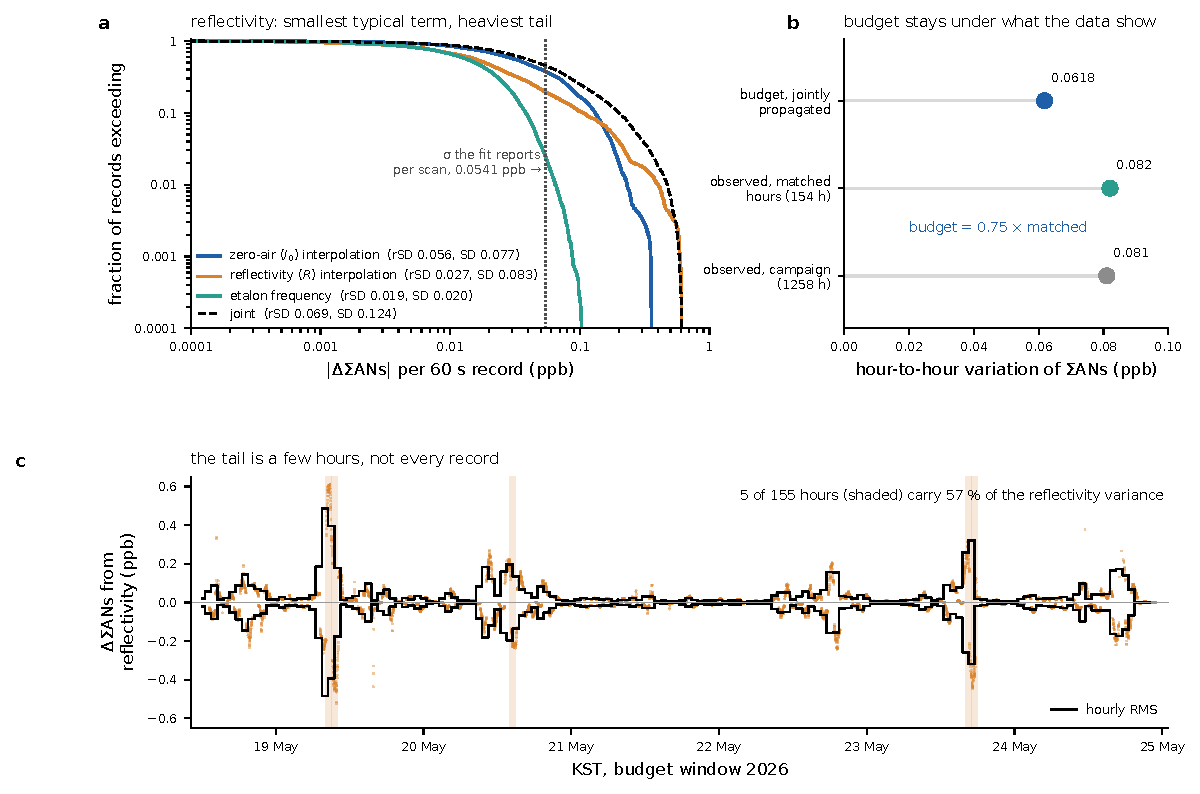
\includegraphics[width=\textwidth]{figures/fig04.pdf}
\caption{Structural error budget of the alkyl nitrate product over the \fieldnum{8847} records of 18--24 May ($g' =
\fieldnum{0.9524}$). \textbf{(a)} Fraction of records whose $\Sigma$ANs changes by more than a given amount for each reference term
alone and all three jointly; legend: robust scale and standard deviation (Table~\ref{tab:2}); dotted: the per-scan fit
uncertainty. \textbf{(b)} Hour-to-hour variation predicted by the joint budget and observed in the matched hours and over
the campaign. \textbf{(c)} Reflectivity term per record (points) and hourly RMS (steps); shaded, the five hours that carry
\fieldnum{57}\,\% of its variance.}
\label{fig:4}
\end{figure*}

The budget describes the instrument when its calibration is working. A perturbation experiment can only be run on
scans that have neighbouring knots of both reference types, so periods in which the calibration itself failed, which
are the periods with the largest errors, are absent from it. The budget window is the best-covered stretch of the
deployment, with no record outside the knot range and no gap longer than two hours; over the campaign \fieldnum{11.03}\,\% of
cold records lie in such gaps (Sect.~\ref{sec:5.3}).

Against what the fit reports, the budget is large. A budget record is one 60\,s ambient bin, which at the
operational scan rate is one scan, and the median fit-propagated $\Sigma$ANs uncertainty at that resolution, over the
same records, is \fieldnum{0.0541}\,ppb. The structural contribution alone is therefore \fieldnum{1.28} times the reported sigma on the
robust scale and \fieldnum{2.29} times it in standard deviation. The total uncertainty is \fieldnum{1.63} to \fieldnum{2.50} times what the
fit reports, the range spanning the two scales rather than any doubt about the measurement. Because
leave-one-out doubles the interpolation interval (Sect.~\ref{sec:4.2}), these are upper-bound estimates for the
interpolation terms in the best-calibrated week of the deployment. They exclude terms common to all knots (cross
sections, Rayleigh scattering, the reflectivity scale) and periods of failed calibration, and are not a campaign-wide bound. The per-scan fit uncertainty is the
appropriate denominator; the uncertainty column shipped with the product, the five-minute fit uncertainty and the
zero-air scatter answer different questions (Appendix~\ref{app:D}, Table~\ref{tab:denominators}).

\subsection{Consistency with the observed variation}
\label{sec:4.5}

The budget can be checked against the data it claims to describe. A channel-differential term must appear in the
channel-difference product, and a term that varies on the timescale of the calibration interval must appear in the
hour-to-hour variation of that product. The observed variation is an upper bound on the measurement error, because
it also contains atmospheric variability. Both sides pass through the same estimator,
$1.4826\,\mathrm{median}|\Delta|/\sqrt{2}$ over adjacent hourly means, and the budget series is itself hourly (median
spacing \fieldnum{1.00}\,h, $p_{90}$ \fieldnum{1.03}\,h), so the comparison is made on the same timestamps, paired
(Table~\ref{tab:hourly_check}). The lag-1 autocorrelation is \fieldnum{$-0.60$} for the budget, because removing a knot pins the interpolant at the two
neighbours and forces it to depart on alternate sides, and \fieldnum{$+0.73$} for the observation in the matched hours, from
atmospheric persistence.

\begin{table}[t]
\caption{Hour-to-hour variation of hourly $\Sigma$ANs, summarised by $1.4826\,\mathrm{median}|\Delta|/\sqrt{2}$ (ppb), observed and predicted by the budget, and the ratio of the budget to the observed statistic in the matched hours.
Observed: the clock-aligned $\Sigma$ANs product (quality flag below 2), hourly means of at least 8 records.}
\label{tab:hourly_check}
\begin{tabular}{lll}
\tophline
 & gate statistic (ppb) & ratio \\
\middlehline
observed, campaign (\fieldnum{1258}\,h) & \fieldnum{0.081} & -- \\
observed, hours matched to the budget (\fieldnum{154}\,h) & \fieldnum{0.082} & -- \\
budget, hourly, jointly propagated, matched hours & \fieldnum{0.0618} & \fieldnum{0.75} \\
budget, at record resolution & \fieldnum{0.0693} & \fieldnum{0.84} \\
\bottomhline
\end{tabular}
\end{table}

The budget predicts \fieldnum{0.75} times the observed hour-to-hour variation (Fig.~\ref{fig:4}b), evaluated on the same
\fieldnum{154} matched hours and \fieldnum{153} consecutive pairs against \fieldnum{0.082}\,ppb; the campaign-wide denominator gives almost the same
ratio, \fieldnum{0.76}. The budget is not larger than the observed variation, as it must be, nor so far below it as to imply an undescribed
dominant error; we assign no pass or fail. The test assumes the error is white at one-hour lag, so any slower
structural component is invisible to it; it cannot separate measurement error from atmospheric variability; and
the upper bound doubles the interpolation interval by construction. The choice of operator alone moves the ratio
from \fieldnum{0.75} to \fieldnum{0.84} (Table~\ref{tab:hourly_check}), which sets the resolution of the method.

Correcting the observed increment statistic for its own lag-1 autocorrelation would defeat the test. Since
$\operatorname{Var}(\Delta) = 2\sigma^2(1-\rho)$ is an identity when $\rho$ is the lag-1 autocorrelation of the same
series, the correction returns the standard deviation of the observed series itself, \fieldnum{0.366}\,ppb for the hourly
$\Sigma$ANs, which is the full geophysical variability that the differencing was introduced to remove.

\subsection{Relation to previous uncertainty treatments}
\label{sec:4.6}

Broadband cavity-enhanced instruments usually report a precision from the spectral fit or from repeated
measurements, and an accuracy assembled in quadrature from campaign-constant terms. \citet{Washenfelder_2008} derive
the mirror reflectivity from the Rayleigh scattering of helium and zero air and bound the absolute accuracy by the
uncertainties of the Rayleigh and absorption cross sections, pressure and temperature, summed in quadrature to a
slope uncertainty of $\pm$4.6\,\% for NO$_2$. \citet{Min_2016} use the same scheme, with an NO$_2$ accuracy of 5.0\,\%
limited mainly by the absorption cross sections. \citet{Nam_2022} give 2.2\,\% for the reflectivity estimate,
dominated by the 2\,\% uncertainty of the zero-air Rayleigh cross section, and 5.2\,\% for the effective path length.
In each case the reflectivity enters as a scale factor with a fixed relative uncertainty. The structural budget
measures a different quantity: the record-to-record error produced by interpolating intermittently measured
references, which is neither a constant scale nor visible in the residual. It adds to the cross-section and Rayleigh
terms, which remain multiplicative and are not re-estimated here.

Residual-based error estimates address a third quantity. \citet{Platt} set out the conditions under which the
least-squares error holds, and corrections such as the correlation factor of \citet{Stutz_1996}, which accounts for
random residual structures and the wavelength-mapping correction, and the bootstrap and Monte Carlo estimates of
\citet{Hausmann_1999} address structure that appears in the residual. The structural terms here leave the residual
unchanged (Sect.~\ref{sec:4.1}), so an inflation derived from the residual should not recover them. We tested this with
the sandwich covariance of Sect.~\ref{sec:3.4}, which removes the correlated-noise deficit of the benchmark. On the budget
records the residual is nearly white (median lag-one autocorrelation \fieldnum{0.06} at 300\,$^{\circ}$C and \fieldnum{0.01} at
180\,$^{\circ}$C); the correction raises the median $\Sigma$ANs sigma by \fieldnum{12}\,\%, and the structural terms remain \fieldnum{1.14} (robust
scale) to \fieldnum{2.03} (standard deviation) times the corrected sigma, against \fieldnum{1.28} and \fieldnum{2.28} before the correction on
the same records. A further step, not attempted here, would treat the zero-air reference and the reflectivity as
measured quantities with their own covariance and propagate the structural term inside the fit rather than
afterwards. What the product should carry in consequence is specified once, in Sect.~\ref{sec:6.1}.
